\chapter{Introduction}
\label{sec:intro}
\section{Introduction}

In this section some common quantities useful for describe the density profiles
are defined and explained.

\subsection{Critical density of the Universe:}

The Critical density of the universe is defined as:

\begin{equation}
\rho_c = \dfrac{3H^2}{8 \pi G}
\end{equation}

Where $H$ is the Hubble parameter and this parameter depends on the cosmological parameters.
This density ...

\subsection{Virialization}

A dark matter halo is virialized when it is in equilibrium, such
an equilibrium occurs after the dark matter have collapsed and
the force of gravity equals the \textbf{relaxation} processes
\citep{BinneyTremaine08}. This happens when the dark matter
reach an overdensity value $\Delta_{vir}$. This overdensity corresponds
to a radius and a mass $r_{vir}$ \& $M_{vir}$ respectively.

 $\Delta_{vir} = \frac{\rho_{vir}}{\rho_c}$.
For a cosmolgy with ($\Omega_m + \Omega_{\Lambda} = 1$) the
solution for the \textbf{Top Hat} model can be  approximated by:

\begin{equation}
\Delta_{vir} = (18 \pi^2 + 82x - 39x^2)/\Omega(z) 
\end{equation}

\citep{EkeColeFrenk96,BryanNorman98} Where $x=\Omega(z)-1$.
For the present time ($z=0$)  $\Delta_{vir}=360$.

The behavior of this function is shown in Fig.\ref{fig:dvir}

\begin{figure}[H]\label{fig:dvir}
\centering
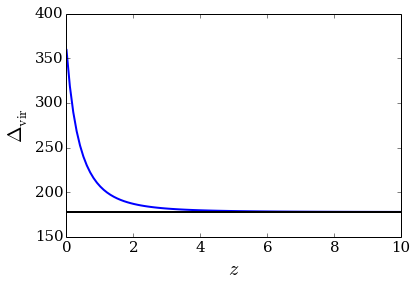
\includegraphics[scale=0.5]{../figures/deltavir.png}
\caption{The solid blue line shows the behaviour of $\Delta_{vir}$
as function of the redshift. The black line show the value of
$\Delta_{vir}=173$ at $z>4$}
\end{figure}

The virial density now can be expressed in terms of $\Delta_{vir}$:

\begin{equation}\label{eq:rhovir}
\rho_{vir} = \frac{3M_{vir}}{4 \pi r_{vir}^3} = \Delta_{vir} \Omega_m \rho_{crit} 
\end{equation}

Where $\Omega_m$ is the density parameter that give as the abundance of matter in the
Universe, it is define as $\Omega_m = \rho / rho_c$ and the actual value is $\Omega_m \simeq 0.3$
Once the virial density is defined with \ref{eq:rhovir} for a given $z$ then the radius
and the virial mass can be related:

\begin{equation}
r_{vir} = \left( \frac{3M_{vir}}{4 \pi \Delta_{vir} \Omega_m \rho_{crit} } \right )^{1/3}
\end{equation}

For example for a halo of mass $M = 1 \times 10^{12}M_{\odot}$ the corresponding radius
is $r_{vir}=262.4$ Kpc
\subsection{$r_{200}$ \& $M_{200}$}

There is another radious and mass of particular interest. This is the radius that enclosed a density
of 200 times the density of the Universe. $M_{200}$ is defined as:

\begin{equation}\label{eq:m200}
M_{200} = 200 \rho_c \dfrac{4}{3} \pi r_{200}^3
\end{equation}

In the same way $M_{vir}$ is defined as:

\begin{equation}\label{eq:mvir}
M_{vir} = \Delta_{vir} \Omega_m \rho_c \dfrac{4}{3} \pi r_{vir}^3
\end{equation}

The critial density $\rho_c$ is the same for both cases, then it is possible
to relate both masses from Eq\ref{eq:m200} and Eq\ref{eq:mvir} as follows:

\begin{equation}
\dfrac{M_{200}}{M_{vir}} = \left(  \dfrac{200}{ \Delta_{vir} \Omega_m}  \right) \left( \dfrac{r_{200}}{r_{vir}}  \right)^3
\end{equation}

Here is common to call $q = \left(  \dfrac{200}{ \Delta_{vir} \Omega_m}  \right) $,  at $z=0$ $q=2.053$.

\begin{equation}\label{eq:q}
\dfrac{M_{200}}{M_{vir}} = q \left( \dfrac{r_{200}}{r_{vir}}  \right)^3
\end{equation}

This Eq.\ref{eq:q} relates $M_{vir}$ and $M_{200}$ for a given $r{vir}$ and $r_{200}$.

\begin{figure}[H]
\centering
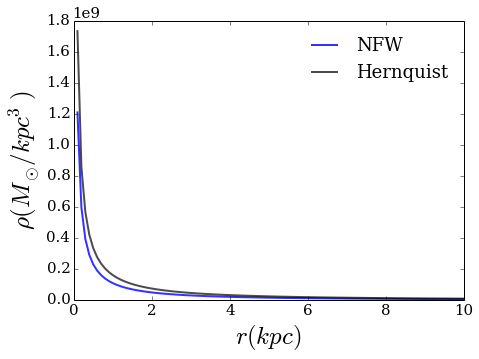
\includegraphics[scale=0.7]{../figures/hernquistNFW.png}
\end{figure}
